
% This file contains your LaTeX preamble. A preamble is a part of your document where all required packages and macros can be defined. This needs to be done before the \begin{document} command.

% Documentclass:
% Standard LaTeX classes are: article, book, report, slides, and letter. These cover the basis, but are not best. More advanced users might want to try out the KOMA classes or the memoir class. Optional arguments: 10pt. The font size of the main content is set to 10pt with the option between [].
\documentclass[11pt]{book}
\usepackage{graphicx}
\let\cleardoublepage\clearpage
% Geometry:
% The papersize of the document is defined with the geometry package. Here, the size is set to A4 with a4paper. Other possibilities are a5paper, b5paper, letterpaper, legalpaper and executivepaper.
\usepackage[a4paper]{geometry}
\newcommand\tab[1][1cm]{\hspace*{#1}}
%removes chapter name from the chapters
\renewcommand{\chaptername}{} 

% AMS math packages:
% Required for proper math display.
\usepackage{amsmath,amsfonts,amsthm}

% Graphicx:
% If you want to include graphics in your document, the graphicx package is required.
\usepackage{graphicx}

% Booktabs:
% The booktabs package is needed for better looking tables. 
\usepackage{booktabs}

% SIunitx:
% The SIunitx package enables the \SI{}{} command. It provides an easy way of working with (SI) units.
\usepackage{siunitx}

% URL:
% Clickable URL's can be made with this package: \url{}.
\usepackage{url}

% Caption:
% For better looking captions. See caption documentation on how to change the format of the captions.
\usepackage{caption}

% Hyperref:
% This package makes all references within your document clickable. By default, these references will become boxed and colored. This is turned back to normal with the \hypersetup command below.
\usepackage{hyperref}
	\hypersetup{colorlinks=false,pdfborder=0 0 0}

% Cleveref:
% This package automatically detects the type of reference (equation, table, etc.) when the \cref{} command is used. It then adds a word in front of the reference, i.e. Fig. in front of a reference to a figure. With the \crefname{}{}{} command, these words may be changed.
\usepackage{cleveref}
	\crefname{equation}{equation}{equations}
	\crefname{figure}{figure}{figures}	
	\crefname{table}{table}{tables}
	


\usepackage{float} 

\usepackage{url} 
\newfloat{fig}{thp}{lof}[chapter]
\floatname{fig}{Figure}



\author{K.J.S. Fernando}
\title{Web of Trust for Better Privacy Protection in Smartphones}
\date{June, 2016}

\newcommand{\namesigdate}[2][5cm]{%
  \begin{tabular}{@{}p{#1}@{}}
    #2 \\[2\normalbaselineskip] \hrule \\[0pt]
    {\small \textit{Signature}} \\[2\normalbaselineskip] \hrule \\[0pt]
    {\small \textit{Date}}
  \end{tabular}
}
\begin{document}
\frontmatter
\begin{titlepage}
\newcommand{\HRule}{\rule{\linewidth}{0.5mm}} % Defines a new command for the horizontal lines, change thickness here

\center % Center everything on the page
 
%----------------------------------------------------------------------------------------
%	HEADING SECTIONS
%----------------------------------------------------------------------------------------

\textsc{\LARGE University of Colombo School of Computing}\\[1.5cm] % Name of your university/college
\textsc{\Large SCS4124 - Final Year Project in Computer Science}\\[0.5cm] % Major heading such as course name

%----------------------------------------------------------------------------------------
%	TITLE SECTION
%----------------------------------------------------------------------------------------

\HRule \\[0.7cm]
{ \huge \bfseries Web of Trust for Better Privacy Protection in Android Applications}\\[0.7cm] % Title of your document
\HRule \\[9cm]

%----------------------------------------------------------------------------------------
%	AUTHOR SECTION
%----------------------------------------------------------------------------------------

\begin{minipage}{0.4\textwidth}
\begin{flushleft} \large
\emph{Researcher:}\\
K.J.S. \textsc{Fernando}\\ % Your name
\emph{Index Number:}\\
12000434
\end{flushleft}
\end{minipage}
~
\begin{minipage}{0.4\textwidth}
\begin{flushright} \large
\emph{Supervisor:} \\
Dr. Kasun \textsc{de Zoysa}\\ % Supervisor's Name
\emph{Co-supervisor:} \\
Mr. Primal \textsc{Wijesekara}
\end{flushright}
\end{minipage}\\[2cm]

%----------------------------------------------------------------------------------------
%	DATE SECTION
%----------------------------------------------------------------------------------------
{\large June, 2016} % Date, change the \today to a set date if you want to be precise


\vfill % Fill the rest of the page with whitespace

\end{titlepage}

%\chapter{Declaration, Abstract and Acknowledgments}
%To be completed.
%\chapter{Declaration}
%\chapter{Abstract}
%\chapter{Acknowledgments}

\tableofcontents

\mainmatter
% The \input{} command reads and processes the indicated example.tex file. Note that docs/ locates the folder where the .tex file is stored.

\chapter*{Acronyms}
\addcontentsline{toc}{chapter}{Acronyms}  
\begin{itemize}
\item[] OS \tab \tab Operating System
\item[] AOSP \tab \tab Android Open Source Project
\item[] Android L \tab Android Lollipop
\item[] Android M \tab Android Marshmallow
\item[] SDK \tab \tab Software Development Kit
\item[] XML \tab \tab Extensible Markup Language
\item[] PGP \tab \tab Pretty Good Privacy
\item[] GPS \tab \tab Global Positioning System
\item[] WiFi \tab \tab Wireless Fidelity
\item[] SSID \tab \tab Service Set Identifier
\item[] RIM \tab \tab Research In Motion
\item[] UID \tab \tab User Identifier
\item[] PIN \tab \tab Personal Identification Number
\item[] UI \tab \tab User Interface
\item[] URL \tab \tab Uniform Resource Locator
\item[] VM \tab \tab Virtual Machine
\item[] HAL \tab \tab Hardware Abstraction Layer
\end{itemize}

\chapter{Introduction} \label{cha:intro}
\section{Preamble}

Android is an open source mobile operating system currently developed and maintained by Google Inc. It was first developed as an advanced operating system for digital cameras, by a team of engineers in Palo Alto, California, and was acquired by Google in 2005. The Android Open Source Project(AOSP) is the collective name for the Linux kernel, middleware components and  applications which form the Android Operating System \cite{a}. Analysis of global smartphone market share indicates that as at March 2016, Android with a market share of 60.99\% is the leading mobile operating system with a lead of 29.23\% over the next most popular operating system, iOS(market share 31.76\%)\cite{b}.
\smallskip

The current version of Android is Android 6.0 M (or Marshmallow), with the SDK version 23. Versions are traditionally named alphabetically after desserts; starting from Cupcake, Doughnut, Eclair to the most recent versions; KitKat, Lollipop and Marshmallow. Each release provides an upgraded version of the OS in terms of software, performance, functionality, features, security and privacy etc.
\smallskip

Users of the Android platform can install "Applications" of different types from digital distribution platforms such as Google Play, Amazon Appstore, SlideME, Mobango etc. As at July 2015, Google's own online marketplace for applications, Google Play, had more then 1.6 million different applications available for download\cite{mil}. Through Google Play, developers can publish and distribute their applications to users of Android compatible smart-phones. When uploading applications, developers are expected to specify which critical resources their applications will need access to in an XML file called the Android Manifest, which is typically found in the root folder of every Android application. Users are required to grant permission for this resource access either before installation(in versions older than Android 5.0) or during runtime(in Android 6.0 and newer devices). 

\section{Background to the Problem}

Users of Android applications are expected to decide on how an application will be allowed to use data without a prior guideline to act as an indicator\cite{felt2011android}. Users are asked to make privacy decisions before they start using the application, at which time they are not equipped with enough knowledge to do so. Up to Android version 5.0(Lollipop) permissions follow a "Do or Die" model, where users are required to grant all the required permissions at install time. Permissions could not be selected or removed individually and choosing not to grant a permission resulted in the application download being canceled. Once installed, app permissions cannot be revoked.
\smallskip 

In versions newer than Android 6.0(Marshmallow) users are allowed to install applications granting selective privacy options, which can later be toggled depending on individual needs. This has mitigated problems that existed in previous versions where users were not given the opportunity to revoke permissions that have already been granted, or choose to grant permission only when required etc. Permissions have been classified based on how "dangerous" they are and certain types of permissions are granted automatically, while other types have to be approved by a user at runtime. The Android framework is built on a Linux kernel, and each application is assigned a UID(Linux User ID) upon installation. Permission requests are connected to the UID, which provides process isolation.
\smallskip



Similar situations with privacy on the internet has brought forth standards such as PGP(Pretty Good Privacy), the concepts of which include "Web of Trust". A Web of Trust is a cryptographic term for a security model where participants authenticate the identity of fellow users.The model in its simplest form is used by social networks including Facebook, LinkedIn and Google+ for user validation and networking\cite{d}. In the context of Android security, there are research applying PGP principles to secure message passing, but not for Application permission privacy configuration\cite{aziz2012android}. 
\smallskip

Android applications require users to approve a list of permissions that will be accessible by the app before installation. This is a shortcoming in an operating system with such a wide user base as users are not equipped with enough knowledge to make a decision, which leads to making uninformed decisions and compromising their own privacy later on since they have no guideline or benchmark available as an indication of how an application will use data once it is downloaded with the necessary permissions granted. Application ratings can be given by users on most marketplaces including Google PlayStore, but this is based on a host of factors which may or may not have taken privacy and security into consideration.

\section{Problem Statement}

\subsection{Privacy and Security}

Privacy and security, although related are different concepts. Privacy is subjective; the user can decide on how private they want their data to be.However security is objective; it is concerned with 'guarding' something that is universally accepted as confidential, such as password, credit card details, pin number etc.
\smallskip

Due to uninformed privacy decisions taken by users when installing apps, both privacy and security are compromised. However security is primarily threatened through malware apps which access permissions without authority, whereas privacy is compromised through users unknowingly granting permissions for applications which then misuse these privileges. Therefore we will be concentrating on privacy violations that occur through permissions which have been granted by users, as there are many research currently focused on malicious code detection and improved security of Android applications.
\smallskip

Users have different needs with regard to privacy, which is why they should be allowed to make their own decisions. Therefore a centralized monitoring system which blocks each privacy infraction would not be ideal since Android does not have information to predict what each user wants beforehand. Privacy infractions are therefore more difficult to predict than security threats, since user preferences also have to be taken into account. Therefore an ideal solution would be to let the users make their own decisions, while providing enough information for them to do so. In the Android platform, users are allowed to make decisions upto a certain extent, but these decisions are usually uninformed since there is no indicator as to what level of privacy will be provided by an application beforehand.

\subsection{Comparison of Application Approval Process}

The leading mobile operating systems apart from Android are iOS by Apple, Windows Mobile and BlackBerry OS. Each of these have different processes and methodologies for developers to follow before submitting an application to the store. A comparison between application submission processes for these platforms shows that each has a centralized process for validation and/or verifying an application before it is made available for users to download. However these processes are usually in place for checking security or applications, and not privacy related issues. 
\smallskip

To submit an application to iTunes, the marketplace for iOS applications, the developer is first required to create an App ID and a Distribution Provisioning Profile and then  submit an application through iTunes connect with detailed information on the app.Three different certificates have to be submitted along with the application; the Distribution Certificate, Push Notification Certificate and Mobile Provisioning Certificate. The app has to be submitted through the Publication Center, where a checklist of complying standards that need to be adhered to has to be filled in.The approval process on average takes six days to one week.\cite{e}
\smallskip

Windows store applications also go through a centralized process before being released. A submission has to be created for each application with a checklist of information. Once the submission is complete and the application has been preprocessed without errors, it is submitted for certification through the Windows Certification Kit. The certification process focuses on three core areas; security tests, technical compliance tests and content compliance tests. The amount of time taken for an application to receive approval fluctuates based factors such as the code and logic complexity, visual content, rating of the developer, other applications in the queue etc. Applications which fail the certification process will be returned with a report indicating where the compliance standards were not met. Developers are allowed to resubmit applications following the same process.\cite{f}
\smallskip

RIM(Research In Motion) BlackBerry requires developers to submit applications for a complex process of reviewing, testing and "readying for publication" before being awarded a Approved/Up For Sale rating. Apps with this rating can be submitted and released on the BlackBerry marketplace; BlackBerry App World.\cite{j} 
\smallskip

Android developers add applications to marketplaces including Google PlayStore, Amazon AppStore, GetJar, SlideMe and F-Droid, which can then be downloaded by users. The problem lies in there being no centralized security measurement for applications on such marketplaces. Developers are trusted to prepare an application for release and then release it through a marketplace, email or website.\cite{g} The Android operating system imposes some security and privacy restrictions, including an install-time permission system, where each application declares what permissions it requires upon installation.\cite{h} This can provide users with control over their privacy since the choice to cancel installation lies with the user.

\subsection{Permission Issues Before Android 6.0}
Up to Android version 5 (Lollipop),users were not given an option to choose which permissions to grant upon application installation. Android v6 (Marshmallow) allows granting and revoking certain permissions upon installation, however, this model is not perfect, and even though it has been almost a year since Marshmallow was launched, it is only running on around 2.3\% of Android devices. \cite{k} The current “all or nothing” model forces users to either refrain from installing an application (no permissions granted) or to grant all permissions requested by an application. This can create problems since studies have shown that users tend to ignore the “grant permission” dialog since they have no choice except to avoid installing the app altogether. \cite{wijesekera2015android} The issue exists for inbuilt applications as well (most of which are classifiable as “bloatware” \cite{mcdaniel2012bloatware} ), for example the Flashlight application inbuilt on devices running HTC’s Android based Sense UI, requests all permissions that can be granted to an application, and since the app is inbuilt there is no way to uninstall/disable it other than rooting the device. 

\subsection{Context of Permission Requests}
In the latest version of Android, Marshmallow, permissions can be toggled. However some issues still exist. 
\smallskip

Research has shown that over 75\% of permission requests rake place while the application is running in the foreground, background or as a service\cite{wijesekera2015android}. The context of a permission access, or specifically the time a permission is requested by an application can contribute towards finding whether the request is legitimate. For example research has further shown that the GPS lication indicator is only visible for 0.04\% of all location access, whereas in reality applications use other permissions such as WifiState to determine the location if a device through SSID information or network tower location. Data collected through such requests breach users privacy and are used for purposes such as targeted marketing \cite{saint201050}.
\smallskip

Research has shown that people are moved to base decisions on what they perceive as the reason for an application to access data\cite{wijesekera2015android}. This may negatively affect the revenue generation model of some applications, since legitimate permission requests, sometimes connected to the revenue generation model of an application, are denied by users who assume that the request malicious. This has affected applications such as AngryBirds, where users have denied the SMS permission to the app, resulting in a failure to unlock levels users have paid for with in-app purchase payments, and even Google's own Google+ application, where thumbnails and images become invisible to users who choose not to grant the Storage permission\cite{u} \cite{w}.
\smallskip

In an ideal situation a user should know why an application is requesting a particular permission; as part of its core functionality, secondary functionality or as a method of revenue generation. However, this is not possible with the current model, since the level of information made available to users regarding application permissions is decided on by the developer. 

\subsection{Other Issues}
This section includes a short summary of existing issues in the Android permission model that will be examined further in chapter two; the literature review.
 
\subsubsection{Permission Creep}
Developers are expected to adhere to the concept of "least privilege" when requesting permissions, namely that only the minimum number of permissions required for an application to function should be requested. This is not always the case, as most developers request permissions which they feel may be required for the applications functionality in future, or just request for unwanted extra permissions due to being unaware or misinformed of these restrictions.

\subsubsection{Capability Leaks}
Capability leaks, also known as permission re-delegation is where an app uses "intents" to exploit the permission granted to another application. In such cases applications do not strictly adhere to their own permissions, but use another more privileged application to access resources. For example when a URL is received through a text message, clicking on it will lead to it being opened in a browser; even though the text message application does not have permission to open URLs it is able to do so by accessing the browser which does have that privilege. 

\subsubsection{Data Availability After Uninstallation}
Upon uninstallation of an application, the Linux UID is recycled and assigned to another application when the device is next rebooted. However research has shown that even though the UID is deleted, the permissions associated with it are not deleted and data still exists as "orphans" without a unique identifier. This may later be exploited by malicious applications which can mimic the UID and access permissions, proving that the consequences of granting permissions can exist even after the application in question is uninstalled from the device. 

\subsection{Problem in Summary}
The current permission model used in Android applications does not include a centralized process for certification or testing before an app is released, and instead relies on the developer to act responsibly and request the least number of permissions that are necessary. However in most cases the privileges given to developers are misused causing capability leaks, permission creep and some other issues, the consequences of which cannot be reversed even after app uninstallation. The simplest way to stop the occurrence of privacy breaches caused by the permission model would be to let the user have more control over permissions to be granted. The problem in a nutshell is that at present users are asked to make uninformed decisions, that can have wide reaching consequences, which they are not equipped to answer.


\section{Research Question}

Different types of interactions take place in this domain; users interact with applications to use the functionality and applications interact with the Operating System to access data(this is where permissions are called on-through the Linux Kernel where a unique user ID is created for each app upon installation). Further, to confirm the level of privacy provided by an app, users could interact with their peers to share the experience of whether the privacy provided by a particular application is adequate or not. Such interactions between applications and the operating system, applications and users, and users and users can be used to create a Web of Trust, focused on creating an improved permission architecture for Android applications and improving flexibility and control for users of the platform. 
\smallskip

Our research goal is to \textbf{propose and evaluate a user-driven privacy model to overcome the problems caused due to improper permission handling in android applications}. 

\section{Goal and Objectives}
\subsection{Goal}
A preliminary step of letting users have more control over granting permissions would be to provide a way for users to determine whether the application keeps to the expected permissions or accesses more than it is supposed to. This is primarily a security issue since apps access permissions without authorization. However some accesses that violate user privacy occur through permissions that \textit{have} been granted by the user. There are many applications to detect unauthorized access and malicious code, but privacy violations occur through accesses that are not unauthorized and are hence not monitored through these applications.Therefore through this research, the expectation is to determine a method through which users will be informed about the trustworthiness of an application based on peer experience with the application.

\subsection{Objectives}
\begin{itemize}
\item Study applications access of permissions
\item Determine a simple scale to rate apps based on privacy breaches that are authorized
\item Determine a method to connect a network of users and assign 'trust' ratings to these users
\item Define threshold values for the 'Web of Trust' including reach of the web, stopping point etc
\item Develop a function to compute the final rating based on the application rating and user's trust rating
\item Present the information in a meaningful way for the user about to install the application
\end{itemize}

\section{Assumptions and Scope}
\subsection{Scope}
The research will focus on Android smartphones with access to the Google PlayStore. Monitoring will be carried out for a selected number of applications from the PlayStore, and not from apps installed using third party websites, promotional links on social media or email, external markets such as the Amazon Appstore, F-Droid etc. The scale to determine trustworthiness of an application will be assigned simply based on factors such as frequency of uninstallation, whether uninstallation happened after a major privacy breach etc. Depending on resource constraints this rating may be equalized to a user assigned rating for an application as well. The information provided to the user will be limited and focused on the core data needed to determine whether an application can be installed without trust issues.
\smallskip 

The research will focus on privacy violations that occur through authorized access. Therefore applications which ask for X permission and then use X to cause some privacy violation will be the focus of this research. We will be operating on the assumptions that trust cannot be misplaced, and that the Linux kernel on which the Android framework is built is completely secure.

\subsection{Delimitation}
The period assigned for the research is limited, and hence the amount of work will be limited by time constraints. Since the purpose is to propose a framework through which information flow to users before installing applications can be improved and not to provide a complete practical implementation of the system, some features will not be included during the research period for clarity and ease of understanding. 
\smallskip

We concentrate the research on the Google PlayStore since different markets follow different methodologies, and monitoring applications downloaded from various sources can lead to malware and security breaches. For the purpose of this research we will assume that the option to install applications from 'Unknown Sources' is disabled.The reasoning for concentrating on privacy is that there are existing research on security violations which occur through an application requesting only permissions X and Y upon installation and then using a loophole to access permission Z without authorization, typically malware and spyware. Further, the information provided will be limited by generated data during the course of analysis, and the ultimate decision on whether or not to install an application will be left to the user. 

\section{Outline of the Thesis} 
To be completed.

\chapter{Literature Review} \label{cha:litrev}
In this chapter we will explore the theoretical background of our work, including research conducted on problems caused by current Android permission models, other solutions found and related work, and applications of trust transitivity in other domains.

\section{The Android Permission Model}
The Android permission model has been developed and updated since the introduction of Android as an operating system. In this section we will examine the theoretical applications of how the permission model is expected to provide privacy and security, and the methods used by similar systems to achieve better privacy protection.

\subsection{Comparison of Application Approval Process}

The leading mobile operating systems apart from Android are iOS by Apple, Windows Mobile and BlackBerry OS. Each of these have different processes and methodologies for developers to follow before submitting an application to the store. A comparison between application submission processes for these platforms shows that each has a centralized process for validation and/or verifying an application before it is made available for users to download. However these processes are usually in place for checking security or applications, and not privacy related issues. 
\smallskip

To submit an application to iTunes, the marketplace for iOS applications, the developer is first required to create an App ID and a Distribution Provisioning Profile and then  submit an application through iTunes connect with detailed information on the app.Three different certificates have to be submitted along with the application; the Distribution Certificate, Push Notification Certificate and Mobile Provisioning Certificate. The app has to be submitted through the Publication Center, where a checklist of complying standards that need to be adhered to has to be filled in.The approval process on average takes six days to one week.\cite{e}
\smallskip

Windows store applications also go through a centralized process before being released. A submission has to be created for each application with a checklist of information. Once the submission is complete and the application has been preprocessed without errors, it is submitted for certification through the Windows Certification Kit. The certification process focuses on three core areas; security tests, technical compliance tests and content compliance tests. The amount of time taken for an application to receive approval fluctuates based factors such as the code and logic complexity, visual content, rating of the developer, other applications in the queue etc. Applications which fail the certification process will be returned with a report indicating where the compliance standards were not met. Developers are allowed to resubmit applications following the same process.\cite{f}
\smallskip

RIM(Research In Motion) BlackBerry requires developers to submit applications for a complex process of reviewing, testing and "readying for publication" before being awarded a Approved/Up For Sale rating. Apps with this rating can be submitted and released on the BlackBerry marketplace; BlackBerry App World.\cite{j} 
\smallskip

Android developers add applications to marketplaces including Google PlayStore, Amazon AppStore, GetJar, SlideMe and F-Droid, which can then be downloaded by users. The problem lies in there being no centralized security measurement for applications on such marketplaces. Developers are trusted to prepare an application for release and then release it through a marketplace, email or website.\cite{g} The Android operating system imposes some security and privacy restrictions, including an install-time permission system, where each application declares what permissions it requires upon installation.\cite{h} This can provide users with control over their privacy since the choice to cancel installation lies with the user.

\subsection{Application Security and Privacy}
The Android OS is built on top of the Linux kernel, which manages the hardware including drivers and power management. From the bottom-up, the next layers include HAL or the Hardware Abstraction Layer, Native libraries and the runtime, which includes the Dalvik virtual machine, the framework with activity managers, system view and content providers, and a layer of applications(Refer Figure 2.1). Each time a new application is installed, the operating system assigns it a unique Linux user ID, which will be persistent for the lifetime of the application on that device. On uninstallation of an application, the user ID will be freed and possibly reassigned to another new application after the device is rebooted for the first time following an uninstallation.
\smallskip 

Permissions are tied to the user IDs, attemting to provide application sandboxing and process isolation by limiting communication between applications to methods overseen by the operating system such as passing of intents. Applications get a dedicated part of the file system connected to its UID whiich can be used to write private data and store databases and raw files, including permission information. According to the description on the Android Security website, the OS "seeks to be the most secure and usable operating system for mobile platforms by re-purposing traditional operating system security controls to protect user data, protext sstem resources and provide application isolation by providing robust security at the OS level through the Linux kernel, mandatory application sandbox for all applications, secure interprocess communication, application signing and application-defined and user-granted permissions"\cite{diagrameka}. However, this system has several loopholes, and malicious applications can access sensitive resources even in cases where sandboxing is done by the user ID system\cite{meshram2014survey}. 
\smallskip
\begin{figure}
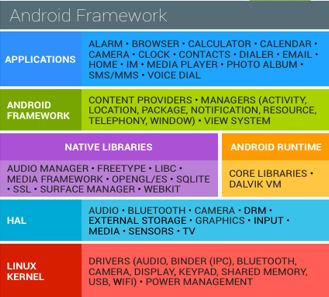
\includegraphics[totalheight=6cm]{Capture1}
\caption{The Android Software Stack}
\end{figure}
\smallskip

\subsection{Installing Applications}
The Android OS allows users to install both free and paid third party Java applications through markets such as Google Play. As discussed Android applications do not go through a review process to measure compliance to guidelines, although most competitors including iOS, Windows and RIM do. Access to sensitive resources, also known as "permissions" are controlled by the operating system to let aplications request access to sysytem functionality through an XML manifest, forming a computer-supported-access-system(CSAS)\cite{stevens2009computer}. Applications are allowed to define their own extra permissions in addition to the 134 core permissions provided by Android\cite{a}. (This research will not focus on third party defined permissions.)
\smallskip

Google Play application listings show information about each application including screenshots, marketing jargon, compatibility with user devices, app information, developer information, content rating, reviews and other related applications. However this does not include a list of permissions used by the app, or any privacy or security related information on the application page. Once a user clicks on the install button, they are expected to approve or disapprove the permission list that appears when downloading on devices older than Android M, without any background information. Permissions and privacy information are not highlighted on both the mobile application of Google Play or the store website\cite{kelley2013privacy}. 

\subsection{Before Android Marshmallow}
Before Android sdk 23, the permission model was based on a "do-or-die" concept. Users were given a list of permissions that would be required upon clicking the "install" link on an application on Google Play. There were no options to grant permissions selectively or revoke when not needed, and choosing not to grant a particular permission resulted in the application installation process being terminated\cite{felt2011effectiveness}. User choice was limited to whether they wanted to use the application, or not, and this has caused habituation even in later versions where permissions can be toggled\cite{wijesekera2015android}, since users choose to approve permissions by reflex as part of the installation process of an application. Research has shown that 83\% of application installations happen without the user consciously reading the permission list\cite{felt2012android}. Android Marshmallow is only being run on 10.1\% of all Android devices according the most current dashboard data at the time of writing\cite{androdashboard}, resulting in many users still being forced to follow the do-or-die model when installing applications(refer figure 2.2). 
%, width=0.5\textwidth
\smallskip
\begin{figure}
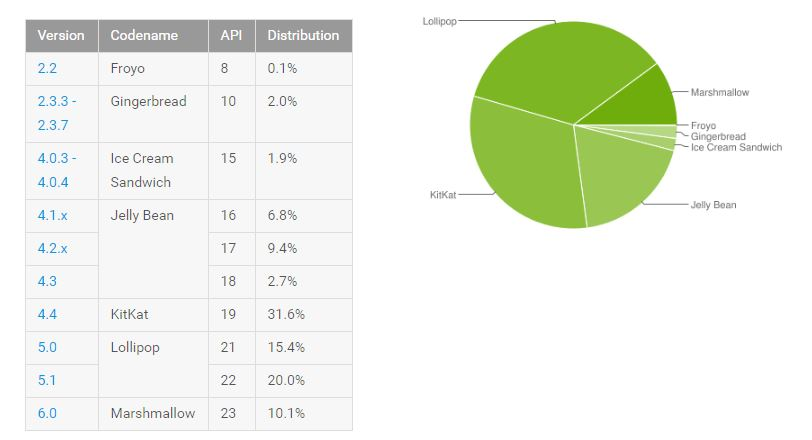
\includegraphics[totalheight=6cm]{Capture2}
\caption{Android Platform Versions as at 30.05.2016\cite{androdashboard}}
\end{figure}
\smallskip

\subsection{After Android Marshmallow}
The current permission model assigns permissions into two categories; normal permissions and dangerous permissions(See Appendix 01 for a list of normal and dangerous permissions). Normal permissions are granted automatically when requested by a user, and can alter basic low-risk elements of a device's settings, such as the display brightness or wallpaper. Dangerous permissions are any permissions that can alter sensitive data on the device or use the device's higher-risk functions, such as connecting to the Internet, and are further classified into groups. If a permission from the same group has previously been approved by the user, then the permission will be automatically granted(i.e. if READ\_SMS permission has been approved by the user then the device will not require permission to access the WRITE\_SMS permission either). However, if a dangerous permission is in a category which has not been approved by the user earlier, a popup notification is generated at runtime, asking the user to approve the permission request. The permission, once granted, can be revoked by toggling a control in the application settings page later on. However, it should be noted that there has been criticism of the classification of permissions, and may researchers such as Felt have pointed out in earlier experiments that the classification should be based on risk to user privacy\cite{felt2011android}, resulting in classification systems that do not correlate with what is currently implemented by Google\cite{androidyearinreview}. Refer figure 2.3 for a flowchart highlighting the recommended model for requesting permission in current Android devices.
\smallskip
\begin{figure}
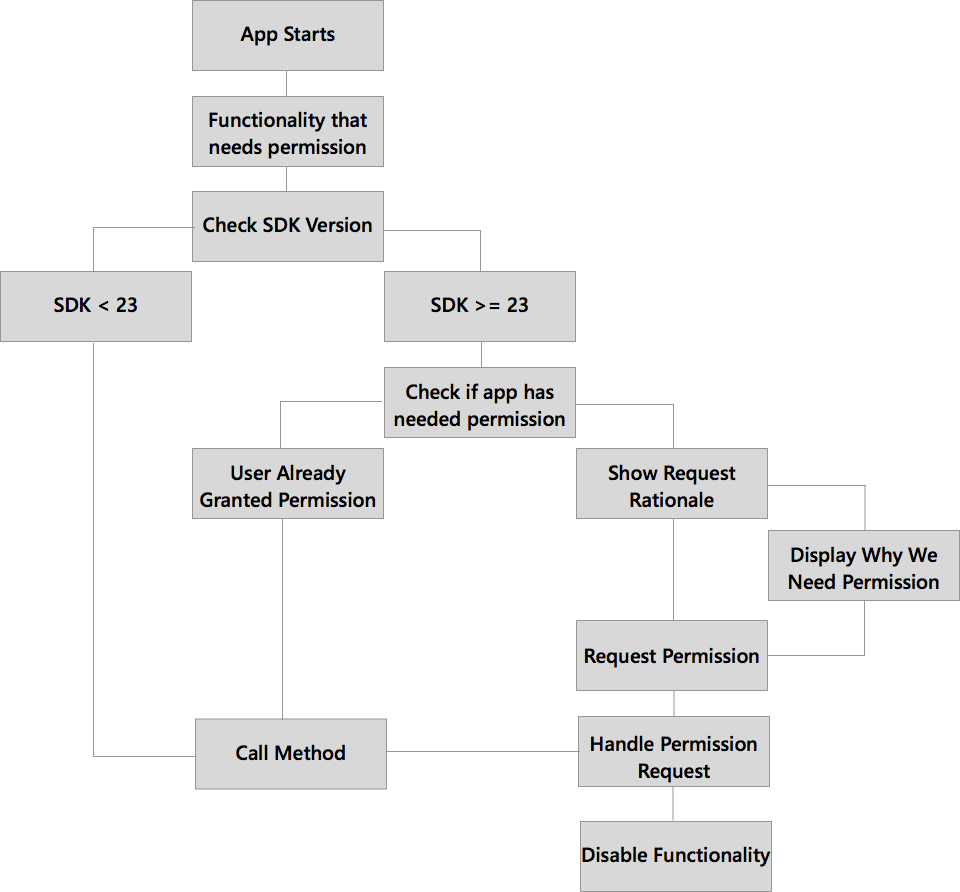
\includegraphics[totalheight=7cm]{Flowchart}
\caption{Android Permission Model- Flowchart\cite{flowchartimage}}
\end{figure}
\smallskip 

\section{Problems with the existing system}
The current permission model is problematic and offers loopholes that can be manipulated to compromise privacy of user data. This section will include a condensed view of research in this domain which highlight and offer solutions to some of these issues. 

\subsection{Least Privilege}
Both the most popular mobile operating systems, iOS and Android, require that developers follow the principle of "least privilege" with regard to permissions. The principle of least privilege states that "Every program and every user of the system should operate using the least set of privileges necessary to complete the job"\cite{schneider2004least}. In the context of Android applications, the principle states that developers should only ask for the very minimum of permissions that are required for the application to function\cite{enck2009understanding}. Applications on the Apple AppStore are screened to check adherence to this principle(and other factors) before being made available for download\cite{gilbert2011vision}. However since there is no such screening process for Android applications, research has shown that these permission guidelines are not generally adhered to by developers\cite{stevens2013asking}. Applications which do follow the permission guidelines are not necessarily popular with users, since permission requests either tend to be ignored due to lack of understanding\cite{felt2011android} \cite{kelley2012conundrum} or granted regardless of whether they are privacy sensitive or not due to habituation\cite{felt2012android}. This results in many popular applications not following the principle of least privilege\cite{wei2012permission}, with research showing that more than 33\% end up asking for more permissions than are required\cite{felt2011android}.

\subsection{Capability Leaks}
Applications can sometimes access permissions which are not requested at install time. Such violations of the permission architecture to access data are referred to as 'capability leaks' \cite{grace2012systematic} \cite{grace2011detecting}. A tool named Woodpecker, which analyzes each application to detect readability of permissions from unguarded interfaces, is frequently used in research in this domain \cite{zhou2012hey}. Through Woodpecker, two different types of capability leaks are identified; explicit leaks which find loopholes and access data without actually requesting permission and implicit leaks which let applications inherit permissions from another application, generally through intents. Other tools used to detect capability leaks include DroidChecker and IntentFuzzer \cite{yang2014intentfuzzer} \cite{chan2012droidchecker}. Capability leaks can also be exploited by malicious applications which use permissions which access permissions which have not been consiously granted to an application by a user for privilege escalation, using this to bypass restrictions on application functionality imposed due to the sand-boxing system\cite{davi2010privilege}.  

\subsection{Data Availability After Uninstallation}
Since application permissions once granted are not revoked even upon uninstallation of an application, the data collected through the permissions granted while the application was installed may still be accessible once the app is uninstalled. Upon uninstallation, the user identity belonging to the application is deleted, but the permissions allowed are not revoked, and data still exists as “orphans” without a unique identifier (or “parent”). These “orphans” may later be exploited by malware causing privacy breaches and leaking of sensitive data \cite{zhang2016life}. Users misunderstanding or choosing not to read permission requests before granting create lasting consequences, the effects of which continue to compromise privacy even after uninstallation of the problematic applications.

\subsection{Permission Creep}
Permission creep occurs in applications that do not follow the principle of least privilege and ask for extra permissions\cite{vidas2011curbing}. Applications may sometimes require permissions that are not required for the core functionality of the application, but rather due to revenue generation methods, since most 'free' applications available on the PlayStore require in-app purchases for extra functionality. Some of these 'free' and low cost applications may sell data to advertisers to generate revenue, without explicit permission from the user. Extra permissions may also be requested in cases where developers have difficulty trying to align permission requests with the functionality required for the application, resulting in genuinely having to request extra permissions that seems unnecessary on analysis, but are mandatory for certain functions \cite{vidas2011curbing}. For example an update for the popular game Angry Birds caused controversy by requesting permission to send SMS messages, which is not part of the expected functionality of the application. However Rovio (the company behind Angry Birds) later explained that this is due to the payment methodology needed to purchase new levels, where an SMS message is sent to Rovio from the device to be billed later by the carrier \cite{w} \cite{u}. 
\smallskip

Studies have shown that over 50\% of applications that request location access do so with the intent of sharing the information with advertisers for targeted marketing\cite{saint201050}. However, completely disallowing such requests would negatively impact the quality of applications available for Android since the revenue generation model would not survive. \cite{aa} In an ideal situation a user should be informed as to why an application is requesting a particular permission; as part of its core functionality, secondary functionality, as a method of revenue generation or any other usage for a permission to be requested. Research has shown that people tend to base their decisions on the reason behind data access\cite{lin2014modeling}. However this is not possible with the current model since the level of information made available to users regarding application permission requests is decided on by the developer.

\section{Proposed Solutions}
Apart from tools developed to identify and provide solutions to the issues discussed above, there have been several research related to alternate models or methodologies that could be followed to mitigate privacy risks in the current model.

\subsection{Facilitating Informed Decisions}
Barerra et al. have suggested hierarchical solutions, recommending a methodology for emperical analysis of permission based security models using Self-Organizing Maps(SOMs), with the intention of identifying potential points of improvement for the current model while increasing information flow conveyed through the permission dialog without creating additional complexity\cite{barrera2010methodology}. Models to breakdown functionality needed by Android applications to create a more fine-grained permission toggle than is available currently has been developed, allowing users to have more control over what data is accessed by an application, and when it is used\cite{bugiel2013flexible}. 
\smallskip

The current model does not allow users access to additional information as to why a particular permission is required, and studies have shown that this could be improved by analyzing human factors more effectively when allowing users to make such decisions. Research which focused on letting users choose applications based on their security and privacy expectations through including a "privacy facts" screen when downloading applications in addition to the list of permissions has proven that decisions made are different when users are given useful privacy information in addition to the current information provided\cite{kelley2013privacy}. Presenting users with personalized examples with their own data has also shown an increase in conscious decision making, and less habituation, for example by showing a sample of the users photos on the device and displaying "if you install this app, it will be able to access and delete the following of your photos" rather than just displaying the CAMERA permission\cite{harbach2014using}. 
\smallskip

Research has been carried out to design methods to recommend applications based on user's history of security and privacy concerns. Systems have been designed to track or reduce privacy violations by recommending applications based on users' security concerns\cite{almohri2014droidbarrier}. Tools have also been developed to track information flow on a device to determine "tainted" information and predict privacy violations in real time\cite{enck2014taintdroid}. Tools such as AppFence which give users the ability to track privacy violations and substitute fake data instead of actual user data for applications which violate privacy conditions have been developed, however this was not successful with all versions of Android and on average only worked for less than 33\% of privacy violations without crashing\cite{hornyack2011these}.

\subsection{Code Analysis to Curb Permission Creep}
Applications requesting unecessary permissions and causing permission creep can be analyzed through static code analysis, by using tools such as pScout\cite{au2012pscout}, and FlowDroid\cite{arzt2014flowdroid}. Static code analysis generally involves reading the Android Manifest and matching permissions which have been requested to those actually used by functions that provide core functionality of the application. Dynamic analysis of applications, runtime monitoring and Java code analysis have also been successful in identifying applications with permission creep \cite{spreitzenbarth2013mobile}. Context of a permission request; time of the request, whether the screen is on or off, whether the application is running visibly as a background or foreground application or service, what the device was displaying while the permission request was taking place, frequency of repitive permission requests(for example searching for network or wifi information) have been shown to influence users when deciding whether a particular permission request is appropriate \cite{wijesekera2015android}. This conforms to Nissenbaum's Theory of Contextual Integrity\cite{nissenbaum2004privacy} with regard to privacy, since the context and flow contribute towards the attitude of a user towards a privacy sensitive request, and not just information such as usage, reason etc.

\section{Transitivity of Trust}
Through this research we will attempt to create a web of trust for users on the Android platform. To our knowledge there are no existing research following this particular approach, however there are research that have been conducted applying PGP models and web of trust to situations which require reputation based trust assessment and user driven models of privacy protection. 

\subsection{Decentralization of Trust}
Donvan et al. have conducted a comprehensive survey on trust models and their applications to the semantic web\cite{artz2007survey}. They have categorized models of trust proposed in previous research into 4 sections:
\begin{enumerate}
\item \textit{Policy-based trust} - Models that are based on the assumption that trust is confirmed by obtaining a sufficient amount of credentials from a single reputable third party. Certificate authorities and other such methods for verifying trust through a centralized method are classified as policy-based trust models.
\item \textit{Reputation-based trust} - These research propose models that use reputation and past actions and connections between entities to assess future behavior and enforce referral based trust or trust through first hand knowledge. Our proposed methods of  using a web of trust classifies as a reputation based trust model.
\item \textit{Generalized models of trust} - Other computable models of trust, some of which cannot be formally verified including research that take psychological factors into consideration when determining trust models are included in this section.
\item \textit{Trust models in information resources} - Trust models developed to verify reliability of information on web sites are included in this section. 
\end{enumerate}
We will be focusing on research that have been conducted on reputation-based models of trust. 

\subsection{Application of Referral Trust in Other Systems}
Research has been conducted into decentralization for reputation management in distributed systems, where peer referrals work to determine the reputation of an entity. Decentralization is viewed as being better than centralization in trust models for distributed systems which need to take human factors into consideration since "with decentralization, each rational entity will be allowed to take responsibility for its own fate, which is a basic human right"\cite{abdul1997using}. Sun et al. propose that in distributed mobile ad hoc networks, trustworthiness plays a role in predicting of and protecting against three types of malicious attacks and decentralized trust models can be used to verify authenticity of nodes rather than a central monitoring system\cite{sun2008defense}.Combining reputation information from another peer, referred to as a "witness"\cite{yu2000social}\cite{yu2002evidential}, to make decisions by distributing reputation information has been followed in several research with decentralized reputation management, and approaches to combine information from an individual and other "witnesses" as a base for decision making in multi-agent systems has been discussed\cite{sabater2002reputation}. Research into computing degrees of trust in case other entities in the network being compromised result in false or conflicting information and application of trust to the peers themselves has been conducted, recommending methods to solve such conflicts in open systems\cite{beth1994valuation}.

\subsection{Trust in Peer Networks}

\subsection{Metrics in a Web of Trust}


\chapter*{Appendix 01}
\addcontentsline{toc}{chapter}{Appendix 01 - Normal and Dangerous Permissions}
\addcontentsline{toc}{section}{Normal Permissions}
\addcontentsline{toc}{section}{Dangerous Permissions}
\section*{Normal Permissions}
\begin{itemize}
\item[] ACESS\_LOCATION\_EXTRA\_COMMANDS
\item[] ACCESS\_NETWORK\_STATE
\item[] ACCESS\_NOTIFICATION\_POLICY
\item[] ACCESS\_WIFI\_STATE
\item[] BLUETOOTH
\item[] BLUETOOTH\_ADMIN
\item[] BROADCAST\_STICKY
\item[] CHANGE\_NETWORK\_STATE
\item[] CHANGE\_WIFI\_MULTICAST\_STATE
\item[] CHANGE\_WIFI\_STATE
\item[] DISABLE\_KEYGUARD
\item[] EXPAND\_STATUS\_BAR
\item[] GET\_PACKAGE\_SIZE
\item[] INSTALL\_SHORTCUT
\item[] INTERNET 
\item[] KILL\_BACKGROUND\_PROCESSES
\item[] MODIFY\_AUDIO\_SETTINGS
\item[] NFC
\item[] READ\_SYNC\_SETTINGS
\item[] READ\_SYNC\_STATS
\item[] RECEIVE\_BOOT\_COMPLETED
\item[] REORDER\_TASKS
\item[] REQUEST\_IGNORE\_BATTERY\_OPTIMIZATIONS
\item[] REQUEST\_INSTALL\_PACKAGES
\item[] SET\_ALARM
\item[] SET\_TIME\_ZONE
\item[] SET\_WALLPAPER
\item[] SET\_WALLPAPER\_HINTS
\item[] TRANSMIT\_IR
\item[] UNINSTALL\_SHORTCUT
\item[] USE\_FINGERPRINT
\item[] VIBRATE
\item[] WAKE\_LOCK
\item[] WRITE\_SYNC\_SETTINGS
\end{itemize}

\section*{Dangerous Permissions}
\begin{itemize}
\item[] READ\_CALENDAR
\item[] WRITE\_CALENDAR
\item[] CAMERA
\item[] READ\_CONTACTS
\item[] WRITE\_CONTACTS
\item[] GET\_ACCOUNTS
\item[] ACCESS\_FINE\_LOCATION
\item[] ACCESS\_COARSE\_LOCATION
\item[] RECORD\_AUDIO
\item[] READ\_PHONE\_STATE
\item[] CALL\_PHONE
\item[] READ\_CALL\_LOG
\item[] WRITE\_CALL\_LOG
\item[] ADD\_VOICEMAIL
\item[] USE\_SIP
\item[] PROCESS\_OUTGOING\_CALLS
\item[] BODY\_SENSORS
\item[] SEND\_SMS
\item[] RECEIVE\_SMS
\item[] READ\_SMS
\item[] RECEIVE\_WAP\_PUSH
\item[] RECEIVE\_MMS
\item[] READ\_EXTERNAL\_STORAGE
\item[] WRITE\_EXTERNAL\_STORAGE
\end{itemize}


\addcontentsline{toc}{chapter}{References}
\bibliographystyle{plain}
\bibliography{refs/references}

\end{document}